\documentclass[a4paper, 8pt]{article}
\usepackage[utf8]{inputenc}
\usepackage[T1]{fontenc}
\usepackage[svgnames]{xcolor}
\usepackage{multicol}
\usepackage{amsmath,amssymb,amsthm}
\usepackage{makeidx}
\usepackage[frenchb]{babel}
\usepackage{bbding}
\usepackage{bm}
%\usepackage{bbm}
\usepackage{fullpage}
\usepackage{enumitem}
\usepackage{hyperref}
\hypersetup{
    colorlinks=true,
    linkcolor=blue,
    filecolor=magenta,      
    urlcolor=red!60!black,
}
\usepackage[tikz]{bclogo}
%\usepackage{lipsum}
\usepackage{xspace}
\usepackage{graphicx}
\usepackage{tikz-cd} %diagrammes commutatifs%
\usepackage{verbatim}
\usepackage{stmaryrd}
\usepackage{cancel}


\usepackage{fancyhdr}

\theoremstyle{definition}
\newtheorem{exo}{Exercice}[section]
\newtheorem{lem}{Lemme}[section]
\newtheorem{thm}{Théorème}[section]
\renewcommand{\headrulewidth}{0.4pt}

\fancyhead[L]{~}
\fancyhead[R]{~}
\fancyfoot[C]{~}
\fancyfoot[R]{Retourner SVP}


\DeclareMathOperator{\ord}{ord}
\DeclareMathOperator{\pgcd}{pgcd}
\DeclareMathOperator{\pg}{\wedge}

\colorlet{greenCom}{green!60!black}
\colorlet{redStruc}{red!80!black}
\date{}
\author{~}
\begin{document}


\everymath{\displaystyle}
\section*{\textcolor{redStruc}{L Codent L Créent - Mémo Processing}}


\begin{bclogo}[logo = \bclampe, arrondi = 0.1, barre=none, epBord = 0.2]{\textcolor{redStruc}{Liens et astuces}}
\begin{itemize}[font= \color{redStruc} \small , label = \textbullet ]
\item \colorbox{yellow!50}{
Comment accéder aux séances? C'est simple! Recopier l'url:   \url{www.tinyurl.com/LCLC2019}}
\item Comment sauvegarder votre travail ? Recopier l'url:   \url{www.tinyurl.com/LCLCsave}. 
Dans la case Identifiant : \textit{LcodentLcreent} et dans la case Mot de passe : \textit{lclc2019}. Cliquer sur \textit{Tableaux} en haut de la page puis trouver votre prénom. Cliquer sur le + en bas à droite puis sur \textit{Note textuelle}. Copier votre code, puis cliquer sur \textit{Enregistrer} en bas à droite.
\item Vous venez d'effacer votre code? Le raccourci \texttt{ctrl + Z} permet d'annuler la dernière action faite (écriture, effacement...)
\item Vous cherchez une couleur en particulier ? Recopier l'url:  \url{https://htmlcolorcodes.com/}
\item \bcattention Pensez à \textbf{enregistrer} vos travaux sur un éditeur (bloc-note, libre office) avant de \textbf{fermer l'onglet de l'activité}, sinon vous perdez le code :) (idem actualisation, etc)
\end{itemize}
\end{bclogo}

\subsection*{Structure de base, coordonnées, formes.}


%%%%%%%%%%%%%%%% 1 %%%%%%%%%%%%%%%%%%%


%\paragraph*{\textcolor{red!80!black}{\bccrayon Structure}}

\begin{bclogo}[logo = \bccrayon, arrondi = 0.1, noborder = true]{\textcolor{redStruc}{Structure}}
\begin{itemize}[font= \color{redStruc} \small , label = \textbullet ]
\item  \texttt{ setup(): \\ \textcolor{white}{bl}Instruction à exécuter.\\ \textcolor{white}{l}run()}
\item \texttt{\textcolor{greenCom}{$\#$ Ceci est un commentaire sur une ligne}}.
\\Il ne sera pas lu/exécuté par l'ordinateur ;) C'est votre mémo.
\end{itemize}
\end{bclogo}
%%%%%%%%%%%%%%% 2 %%%%%%%%%%%%%%%%%%%


\begin{bclogo}[logo = \bccrayon, arrondi = 0.1, noborder = true]{\textcolor{redStruc}{Système de coordonnées}}
\begin{itemize}[font= \color{redStruc} \small , label = \textbullet ]
\item Les axes x et y ne sont pas les mêmes que d'habitude: ~\\\begin{minipage}[l]{.6\linewidth}
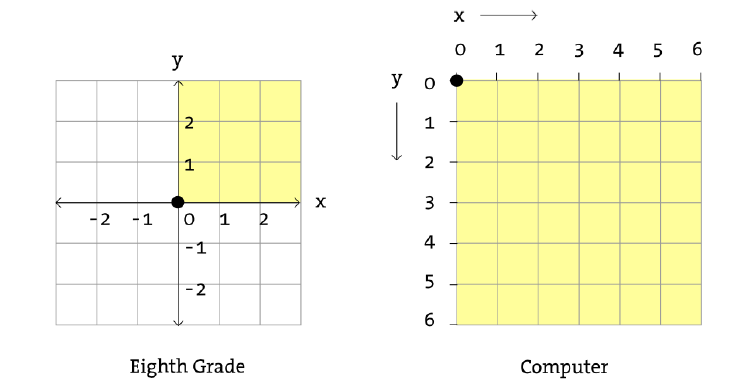
\includegraphics[scale=0.3]{systemecoordonneesprocessing.png}
\end{minipage}
\begin{minipage}[r]{.3\linewidth}
\item Le point du coin en haut à gauche de chaque fenêtre est à la coordonnées $(0,0)$.  La fonction \texttt{transtion()} change cet axe.\\
\item Unité de mesure: \textbf{pixel}.
\end{minipage}
\item \texttt{width}: Longueur (L) de l'objet, \textcolor{redStruc}{\small \textbullet} \texttt{height}: Hauteur (H) de l'objet.
\item \texttt{size(width, height)}: Règle la taille $(L, H)$ de la fenêtre principale.

\end{itemize}
\end{bclogo}

%%%%%%%%%%%%%% 3 %%%%%%%%%%%%%%%%%%%%



\begin{bclogo}[logo = \bccrayon, arrondi = 0.1, noborder = true]{\textcolor{redStruc}{Bases de géométrie}}
Les commandes suivantes dessinent...
\begin{itemize}[font= \color{redStruc} \small , label = \textbullet ]
\item \texttt{ellipse$(x,y,l,h)$}: une ellipse en $(x,y)$, de longueur $l$ et de hauteur $h$.
\item \texttt{rect$(x,y,l,h)$}: un rectangle, dont le coin en haut à gauche est en $(x,y)$, de longueur $l$ et de hauteur $h$.
\item \texttt{line$(x_1,y_1,x_2,y_2)$}: un segment, d'extrémité $(x_1,y_1)$ à $(x_2,y_2)$.
\item \texttt{point$(x,y)$}: un point à la coordonnée $\left(x,y\right)$
\item \texttt{triangle$(x_1,y_1,x_2,y_2,x_3,y_3)$}: un triangle dont les coins sont en $(x_1,y_1)$, $(x_2,y_2)$, $(x_3,y_3)$.
\item \texttt{quad$(x_1,y_1,x_2,y_2,x_3,y_3,x_4,y_4)$} un quadrilatère dont les coins sont en $(x_1,y_1)$, $(x_2,y_2)$, $(x_3,y_3)$, $\left( x_4, y_4 \right)$.
\end{itemize} 
%Voici les différentes figures de bases:
%\begin{center}
%\includegraphics[scale=0.5]{figuresdebase.png}
%\end{center}
\end{bclogo}

%%%%%%%%%%% 5 %%%%%%%%%%%%%%%%%%%%%


\thispagestyle{fancy}
\begin{bclogo}[logo = \bccrayon, arrondi = 0.1, noborder = true]{\textcolor{redStruc}{Bordures, remplissage, et contour des formes}}
\begin{itemize}[font= \color{redStruc} \small , label = \textbullet ]
\item Où trouver les codes R-V-B des couleurs? Code déc. du tableau \url{https://fr.wikipedia.org/wiki/Couleur_du_Web#Noms_de_couleurs_SVG_1.0}
\item \texttt{background(color)}: Règle la couleur de fond de la fenêtre principale.
\item \texttt{fill(R,V,B)}: Règle la couleur de fond des prochaines formes à (R,V,B sont des nombres entre $0-255$ et règlent les taux de Rouge, de Vert et de Bleu).
\item \texttt{nofill()}: enlève le fond pour les prochaines formes.
\item \texttt{stroke(R,V,B)}: Règle la couleur de la bordure des prochaines formes (même format que \texttt{fill(R,V,B)}).
\item \texttt{noStroke()}:  Enlève les bordures pour des prochaines formes.
\end{itemize} \end{bclogo}

\subsection*{Des boucles et des tests}

%%%%%%%%%% 6 %%%%%%%%%%%%%%%%%%%%%

\begin{bclogo}[logo = \bccrayon, arrondi = 0.1, noborder = true]{\textcolor{redStruc}{Structure des tests et des boucles}}

\begin{itemize}[font= \color{redStruc} \small , label = \textbullet ]

\item \textbf{Si...alors...}.
\\Ce test permet d'exécuter différentes actions selon des conditions. Voici la structure d'un test:
\\
\texttt{If (une condition):\\
\\ \textcolor{white}{tb}Execution d'un code\\
\\ Elif (une condition):\\\\
\textcolor{white}{tb}Execution d'un code\\
\\ Else (pas besoin de condition):\\\\
\textcolor{white}{tb}Execution d'un code}


\item  \textbf{Boucle for: Pour... faire}
\\La boucle permet de répéter une action sans la ré-écrire:
\\ \texttt{For x in range(TRUC):\\\\
\textcolor{white}{tb}Exécution d'un code}
\item L'exécution du code peut dépendre de \texttt{x}.
\item Dans \texttt{TRUC} on peut mettre:
\begin{itemize}[font= \color{redStruc} \small , label = \textbullet ]
\item $\left(1,12,2\right)$ pour exécuter la commande pour $x=1,3,5,7,9$ (le pas est de $2$).
\\\textit{Exemple: \texttt{print(range(1, 10, 4))} renvoie $\left[ 1,5,9\right]$ }
\item $\left(1,7\right)$ pour exécuter la commande pour $x=1,2,3,4,5,6$
\\\textit{Exemple: \texttt{print(range(1, 10))} renvoie $\left[ 1,2,3,4,5,6,7,8,9\right]$}
\end{itemize}
\item \bcattention \textbf{Dans tous les cas}: L'indentation (=les deux espaces) sont importants.
\end{itemize}




\end{bclogo}

%%%%%%%%% 7 %%%%%%%%%%%%%%%%%%%%%%%


\begin{bclogo}[logo = \bccrayon, arrondi = 0.1, noborder = true]{\textcolor{redStruc}{Opérateurs}}
\begin{itemize}[font= \color{redStruc} \small , label = \textbullet ]
\item \texttt{=}: défini comme. Exemple: \texttt{Taille=6} affecte $6$ à la variable appelée \texttt{Taille}.
\item \texttt{==}: test d'égalité
\item  \texttt{>}: supérieur à. Et bien sûr: \texttt{>=} supérieur ou égal à
\item  \texttt{!=}: test d'inégalité
\end{itemize} 
\end{bclogo}



%%%%%%%%%%%%%%% 8 %%%%%%%%%%%%%%%%%

\subsection*{Un peu d'animation...}

\begin{bclogo}[logo = \bccrayon, arrondi = 0.1, noborder = true]{\textcolor{redStruc}{Affichage et animations}}
\begin{itemize}[font= \color{redStruc} \small , label = \textbullet ]
\item \texttt{frameRate(fps)}: Règle les FPS (Nombres d'images/sec) de l'application.
\item \texttt{print(string)}: Écrit une chaîne de caractère sur la console.
\item \texttt{println(string)}: La même chose, avec un saut de ligne.
\item \texttt{delay(milliseconds)}; Place une pause/un délai (en milisecondes).
\end{itemize}
\end{bclogo}


%%%%%%%%%%%%%% 9 %%%%%%%%%%%%%%%%%%


\begin{bclogo}[logo = \bccrayon, arrondi = 0.1, noborder = true]{\textcolor{redStruc}{Variables globales}}
\begin{itemize}[font= \color{redStruc} \small , label = \textbullet ]
\item \texttt{mouseX, mouseY}: Renvoie les coordonnées (X,Y) de la position de la souris.
\item \texttt{pmouseX, pmouseY}: Renvoie les coordonnées (X,Y) de la position précédente de la souris.
\item \texttt{draw()}: Se place après \texttt{setup()}, on y met les éléments \textbf{animés}
\item \texttt{frameRate}: Règle le nombre d'images par secondes.
\item \texttt{frameCount}: Renvoie le nombre d'images qui ont été affichées par \texttt{draw()}
\end{itemize} 
\end{bclogo}

%%%%%%%%%%%% 10 %%%%%%%%%%%%%%%%%%%%%


Pour le jour $J$, du mois $m$, à l'heure $H$, la minute $M$ et la seconde $S$
\begin{bclogo}[logo = \bccrayon, arrondi = 0.1, noborder = true]{\textcolor{redStruc}{Heure $\&$ Date}}
\begin{itemize}[font= \color{redStruc} \small , label = \textbullet ]
\item \texttt{month()}: Renvoie le mois actuel (format $4$ pour avril par ex.)
\item \texttt{day()}: Renvoie le jour $J$ du mois $m$ actuel.
\item \texttt{hour()}: Renvoie l'heure $H$ actuelle.
\item \texttt{minute()}: Renvoie la minute $M$ actuelle.
\item \texttt{second()}: Renvoie la seconde $S$ actuelle.
\end{itemize} 
\end{bclogo}
\end{document}
